\documentclass[11pt]{article}

\usepackage[margin=1.15in]{geometry}
\usepackage{amsmath}
\usepackage{amssymb}
\usepackage{graphicx}

% One symbol per object, as in notes/correlated_bias_prior_v2.
\newcommand{\Cov}{\mathsf{C}}
\newcommand{\T}{^{\mathsf{T}}}
\newcommand{\kmax}{k_{\rm max}}
\newcommand{\hMpc}{\,h/{\rm Mpc}}
\newcommand{\chidof}{\sqrt{\langle\chi^2\rangle/n_{\rm dof}}}
% The clause every caption that quotes k_max carries.
\newcommand{\kmaxclause}{$\kmax$ quoted at $z = 0$; each bin is cut at
  $\kmax/D(\bar{z}_i)$ by the UV-fraction criterion ($\alpha = 0.05$)
  within the shipped mask.}

\title{Up to which $k_{\rm max}$ is linear galaxy bias enough?}
\date{November 2026}
\author{}

\begin{document}

\begin{center}
  {\LARGE Up to which $k_{\rm max}$ is\\[0.3em] linear galaxy bias enough?\par}
  \vspace{0.6em}
  {\large A linear-bias fit to a one-loop truth on four bin layouts\par}
  \vspace{1em}
  {\large November 2026\par}
\end{center}
\vspace{1em}

\section{Summary}
\label{sec:summary}

\paragraph{The question.}
The forecast fits the DESI galaxy clustering band powers
$C_\ell^{gg}$ of thin redshift bins with linear galaxy bias,
$\delta_g = b_1\,\delta$: the galaxy density contrast $\delta_g$ is
the matter density contrast $\delta$ times one number $b_1$ per bin.
This is exact on large scales.  On smaller scales higher-order bias
terms grow with the wavenumber $k$, so linear bias holds only below
some scale cut $\kmax$.  This note answers two questions about the
four linear-bias priors of the correlated-prior note
(\texttt{notes/correlated\_bias\_prior\_v2}, section ``The models'').
\begin{enumerate}
  \item Up to which $\kmax$ does a linear-bias fit to a one-loop truth
    stay unbiased, on each of four bin layouts?
  \item Does the accuracy test of the linear-bias priors give the same
    verdict for $\Omega_m$ and $A_s$ as for $(w_0, w_a)$?
\end{enumerate}
Here $w(a) = w_0 + w_a(1 - a)$ is the dark-energy equation of state,
with $a$ the scale factor; $\Omega_m$ is the matter density today in
units of the critical density; and $A_s$ is the amplitude of the
primordial curvature power spectrum, sampled as $10^9 A_s$.

\paragraph{The answer.}
\begin{enumerate}
  \item Linear bias is safe only at the smallest scanned cut,
    $\kmax = 0.05\hMpc$, and for every prior and every truth only on
    the layout of equal comoving width.  At $\kmax = 0.075\hMpc$, the
    cut of the correlated-prior note, a linear fit is biased on every
    layout and under every prior, and freeing the bias bin by bin
    does not cure it.  The safe cut keeps $1$--$6\%$ of the
    dark-energy figure of merit.  The correlated-prior note therefore
    carries the higher-order bias at $0.075\hMpc$ with the one-loop
    model A.
  \item Yes.  Scored for $\Omega_m$ and $A_s$, the test excludes the
    growth-tied prior, finds the baseline prior honest only under its
    own scatter, and the pessimistic prior honest under both.
\end{enumerate}

\paragraph{The setup.}
The data are the DESI band powers $C_\ell^{gg}$ alone, computed
without the Limber approximation, for six tracer groups (BGS,
LRG1--3, ELG1--2) on four bin layouts: bins of equal comoving width
$\Delta d_{\rm com} = 62$~Mpc, and bins of fixed redshift width
$\Delta z = 0.02$, $0.05$ and $0.2$.

Each one-loop truth is fitted with linear bias under four priors.
With $D(z)$ the linear growth factor ($D(0) = 1$), $\bar{z}_i$ the
mean redshift of bin $i$ and $B_g$ one amplitude per group $g$, they
are: \textbf{growth-tied}, $b_i = B_g/D(\bar{z}_i)$;
the \textbf{baseline prior}, a free amplitude and tilt per group plus
a residual of width $\sigma_g = 3\%$ for BGS and $1\%$ for the other
groups, correlated over $L = 0.2$ in redshift; the
\textbf{pessimistic prior}, the same with $\sigma_g = 3\%$ everywhere
and $L = 0.05$; and \textbf{free}, one bias per bin with a flat prior.
The Gaussian covariance uses the growth-tied biases and is computed
for $14{,}000$ square degrees, rescaled to the survey's $12{,}300$.

A fit's parameter shift is its Fisher linear response
(Appendix~\ref{app:method}).  The $(w_0, w_a)$ shift is scored in
units of the fit's marginalized error ellipse, and $\Omega_m$ and $A_s$
each in units of its own marginalized error $\sigma$.  A fit is
unbiased when every shift is below $\sigma/3$, the threshold of the
correlated-prior note's accuracy test.

\paragraph{The scale cut.}
$\kmax$ labels one cut per bin.  Bin $i$ is cut at
$\kmax/D(\bar{z}_i)$: matter is less nonlinear at higher redshift, so
the cut moves to higher $k$ as $1/D$.  The cut is the non-Limber
ultraviolet-fraction criterion of Saraivanov et
al.~\cite{Saraivanov2026}, which follows DeRose and
Chen~\cite{DeRoseChen2025}.  Each band power is split into
$C_\ell^{\rm IR}$, from the power spectrum below the bin's cut
wavenumber, and $C_\ell^{\rm UV}$, from the power above it.  A band is
kept while
\begin{equation}
  \frac{|C_\ell^{\rm UV}|}{|C_\ell^{\rm UV}| + |C_\ell^{\rm IR}|}
  \;<\; \alpha = 0.05 ,
  \label{eq:uvfraction}
\end{equation}
and the kept bands are intersected with the shipped mask, which caps
every bin at $k = 0.1185\,{\rm Mpc}^{-1}$ with no growth scaling.  The
scan runs over $\kmax = 0.05, 0.075, \ldots, 0.25\hMpc$, and every
$\kmax$ in this note is the $z = 0$ value.

\paragraph{The truths.}
The truth is model A of \texttt{notes/higher\_order\_bias}, computed
with CosmoLike's one-loop engine.  Its real-space galaxy power
spectrum is
\begin{equation}
  P_{gg}(k) \;=\; b_1^2\,P_{\rm mm}(k)
  \;+\; P_{\rm loop}(k;\, b_1, b_2, b_{s^2})
  \;+\; \alpha_0\,k^2 P_{\rm mm}(k) ,
  \label{eq:modela}
\end{equation}
with $P_{\rm mm}$ the nonlinear matter power spectrum and
$P_{\rm loop}$ the one-loop terms.  These carry the quadratic bias
$b_2$, the response of the galaxy density to $\delta^2$, and the tidal
bias $b_{s^2}$, its response to the squared tidal field.  $\alpha_0$
is the $k^2$ counterterm, in $h^{-2}\,{\rm Mpc}^2$, which absorbs the
small-scale sensitivity of the loops; it multiplies $P_{\rm mm}$,
CosmoLike's convention (DESI multiplies the linear spectrum).  The \emph{calibrated} truth keeps the
fiducial $b_1$, puts $b_2$ on the Lazeyras et al.\ fit $b_2(b_1)$
\cite{Lazeyras2016} and $b_{s^2} = -\tfrac{4}{7}(b_1 - 1)$ on
co-evolution \cite{Saito2014}, and sets the third-order bias
$b_3 = 0$, $\alpha_0 = 0$ and no stochastic term.  Four brackets
offset every group's $b_2$ by $\pm 1$ (``$b_2 \pm 1$'', model A's
prior width) or set $\alpha_0 = \pm 12.5\,h^{-2}\,{\rm Mpc}^2$, the
counterterm prior width of the DESI 2024 full-shape analysis
\cite{DESI2024V}.  ``Every truth'' means all five.

\paragraph{The safe cut, layout by layout.}
Table~\ref{tab:safe} lists the largest safe $\kmax$: the largest
scanned cut at which every shift stays below $\sigma/3$, at that cut
and at every smaller cut that has a fit.  Figure~\ref{fig:fobkmax}
draws the shifts against $\kmax$.
\begin{itemize}
  \item $\Delta d_{\rm com} = 62$~Mpc: safe at $0.05$ under every
    prior and for every truth; the largest shift at that cut is
    $0.14\sigma$.
  \item $\Delta z = 0.02$: fails.  At $0.05$ the ultraviolet-fraction
    criterion keeps no band of any spectrum, so there is no fit; at
    $0.075$ every prior fails.
  \item $\Delta z = 0.05$: safe at $0.05$ for every truth under the
    growth-tied and baseline priors (largest shift $0.28\sigma$).  The
    pessimistic prior passes for the calibrated truth only, and fails
    the brackets $b_2 - 1$ and $\alpha_0 = -12.5$ with $(w_0, w_a)$
    shifts of $0.42$ and $0.44$.  The free prior fails already for the
    calibrated truth ($0.36$).
  \item $\Delta z = 0.2$: safe at $0.05$ for the calibrated truth under
    every prior, but no prior passes every truth: $b_2 - 1$ and
    $\alpha_0 = -12.5$ shift $(w_0, w_a)$ by up to $0.49$
    (growth-tied) and $0.59$ (the other priors).  Its groups hold one
    or two bins each, so the free amplitude and tilt already free
    every bin, and the baseline, pessimistic and free priors coincide.
\end{itemize}
In every fitted case at $0.05$ the largest shift comes from a negative
bracket, $b_2 - 1$ or $\alpha_0 = -12.5$.

\begin{table}[ht]
  \centering
  \begin{tabular}{lcccc}
    \hline
    Layout & growth-tied & baseline & pessimistic & free \\
    \hline
    $\Delta d_{\rm com} = 62$~Mpc & $0.05$ / $0.05$ & $0.05$ / $0.05$
      & $0.05$ / $0.05$ & $0.05$ / $0.05$ \\
    $\Delta z = 0.02$ & fails / fails & fails / fails
      & fails / fails & fails / fails \\
    $\Delta z = 0.05$ & $0.05$ / $0.05$ & $0.05$ / $0.05$
      & $0.05$ / fails & fails / fails \\
    $\Delta z = 0.2$ & $0.05$ / fails & $0.05$ / fails
      & $0.05$ / fails & $0.05$ / fails \\
    \hline
  \end{tabular}
  \caption{The largest safe $\kmax$ [$h$/Mpc] of a linear-bias fit to
    the one-loop truth, as ``calibrated truth / every truth''.
    ``fails'': the smallest fitted cut already fails ($0.075$ on
    $\Delta z = 0.02$, where $0.05$ keeps no band).  \kmaxclause}
  \label{tab:safe}
\end{table}

\begin{figure}[t]
  \centering
  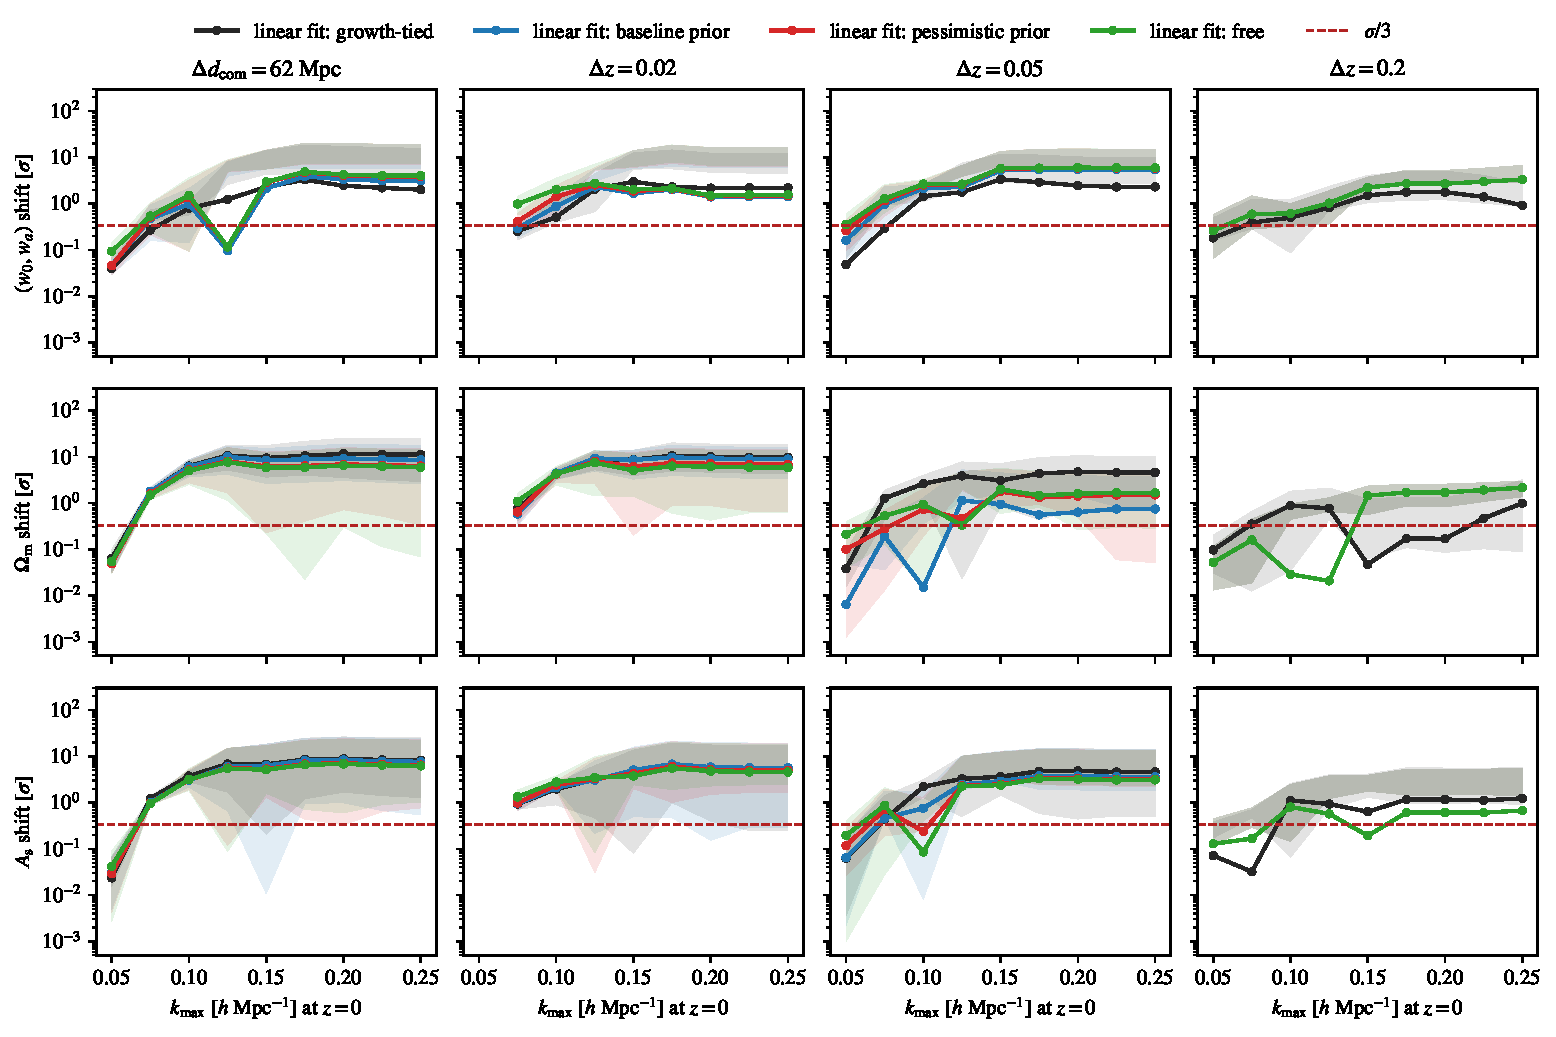
\includegraphics[width=\linewidth]{plots/fob_kmax/fob_kmax.pdf}
  \caption{The shift of a linear-bias fit to the one-loop truth
    against the scale cut.  Columns: the bin layouts.  Rows: the
    $(w_0, w_a)$, $\Omega_m$ and $A_s$ shifts (Appendix~\ref{sec:scores}).
    Lines: the calibrated truth, one color per linear-bias prior.
    Bands: the range of the four brackets.  Dashed line: $\sigma/3$.
    On $\Delta z = 0.02$ the cut at $0.05$ keeps no band.  On
    $\Delta z = 0.2$ the free line covers the baseline and pessimistic
    ones.  \kmaxclause}
  \label{fig:fobkmax}
\end{figure}

\paragraph{At $\kmax = 0.075\hMpc$ every prior is biased.}
For the calibrated truth the largest shift ranges from $0.40\sigma$
($\Delta z = 0.2$, growth-tied) to $1.8\sigma$
($\Delta d_{\rm com} = 62$~Mpc).  On $\Delta d_{\rm com} = 62$~Mpc
the four priors move $\Omega_m$ by $1.5$--$1.8\sigma$, $A_s$ by
$1.0$--$1.3\sigma$ and $(w_0, w_a)$ by $0.28$--$0.55$; the step from
$0.05$ to $0.075$ multiplies the shifts by factors of $6$ to $53$.

\paragraph{Why more bias freedom does not help.}
A linear bias multiplies a bin's power spectrum by the constant
$b_i^2$ at every $k$.  The loop terms and the counterterm of
Eq.~\eqref{eq:modela} have other shapes, so inside one bin the truth
differs from every linear model by a scale dependence that no choice
of $b_i$ removes.  The fit pushes that residual into the cosmological
parameters, which do change the shape of the band powers.  Freeing
the biases changes which parameter takes the residual, not whether
one does.  On $\Delta d_{\rm com} = 62$~Mpc at $0.075$, going from
the growth-tied to the free prior lowers the $\Omega_m$ shift from
$1.82$ to $1.53$ and raises the $(w_0, w_a)$ shift from $0.28$ to
$0.55$.  On $\Delta z = 0.05$ the baseline prior moves the error from
$\Omega_m$ ($0.19$, against $1.33$ for growth-tied) to $(w_0, w_a)$
($0.97$, against $0.31$).

\paragraph{The accuracy test for $\Omega_m$ and $A_s$.}
Figure~\ref{fig:ladderbiasparams} repeats the accuracy test of the
correlated-prior note with linear-bias fits and linear truths at
$\kmax = 0.075\hMpc$.  Each truth is a known bias drift (the
$r < 19.5$ flux limit in BGS, a conserved galaxy population in the
other groups) plus a residual drawn from the baseline or the
pessimistic prior: $2000$ draws, each fitted under every prior.  The
statistic is $\chidof$, where $\chi^2$ is the squared distance of the
recovered parameters from the truth in units of the fit's marginalized
covariance, $n_{\rm dof} = 2$ for $(w_0, w_a)$ and $1$ for $\Omega_m$
or $A_s$, and $\langle\cdot\rangle$ averages over the random truths
and the data noise.  It asks, for each parameter, whether the fit's
quoted error bar honestly covers where the fit actually lands: $1$
means it does, and above $1$ it is the factor by which the error bar
is too small.  It scores the recovered parameters, not the $\chi^2$
of the data: a biased fit can match the band powers well while its
cosmology is wrong.

The verdict for $\Omega_m$ and $A_s$ is the verdict for
$(w_0, w_a)$:
\begin{itemize}
  \item \textbf{growth-tied} is excluded: the conserved-population
    drift alone shifts $(w_0, w_a)$ by $5.0$--$11.6$ and $\Omega_m$ by
    $0.48$--$6.2\sigma$ across the layouts;
  \item the \textbf{baseline prior} gives $\chidof = 1$ under its own
    scatter (at most $1.02$), but under pessimistic scatter its error
    bars are too small by up to $1.65$ for $(w_0, w_a)$, $2.0$ for
    $\Omega_m$ and $1.48$ for $A_s$ ($\Delta z = 0.05$);
  \item the \textbf{pessimistic prior} is honest or conservative under
    both truths, with $\chidof \le 1.05$;
  \item \textbf{free} recovers every such truth exactly.
\end{itemize}
Every value is in \texttt{plots/ladder\_bias\_params/data.json}.

\begin{figure}[!t]
  \centering
  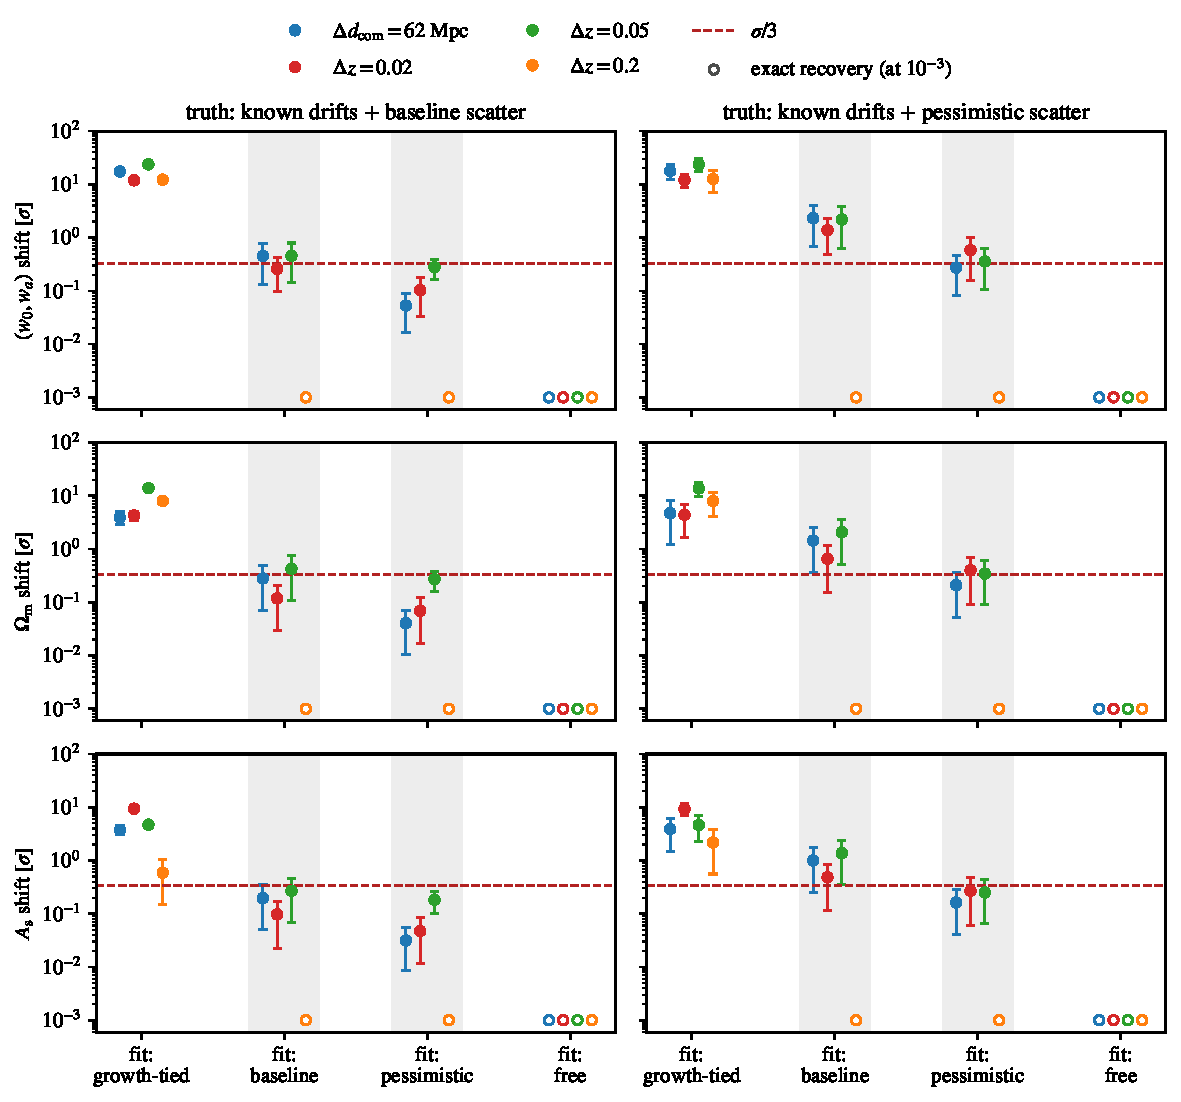
\includegraphics[width=0.8\linewidth]{plots/ladder_bias_params/ladder_bias_params.pdf}
  \small
  \caption{The accuracy test of the linear-bias priors, scored for
    $(w_0, w_a)$, $\Omega_m$ and $A_s$.  Truths: the growth-tied bias
    times $1 + \delta_i^{\rm drift} + \varepsilon_i$, with the known
    drift $\delta_i^{\rm drift}$ and a residual $\varepsilon_i$ drawn
    from the baseline (left) or the pessimistic prior (right).  Each
    truth is fitted under every prior (horizontal axis).  Points: the
    mean shift over the truths; bars: 16th--84th percentiles; colors:
    the layouts; dashed line: $\sigma/3$; gray columns: the baseline
    and pessimistic priors.  Where the fit's prior equals the truth's
    scatter, the fit's error covers the mean shift and $\chidof = 1$.
    Open markers at $10^{-3}$: exact recovery.  \kmaxclause}
  \label{fig:ladderbiasparams}
\end{figure}

\paragraph{The price of the safe cut.}
Figure~\ref{fig:fomkmax} draws, for the three priors that pass the
accuracy test, the dark-energy figure of merit against $\kmax$:
\[
  {\rm FoM}(w_0, w_a) \;=\; [\det \mathrm{Cov}(w_0, w_a)]^{-1/2} ,
\]
the inverse area of the marginalized $(w_0, w_a)$ ellipse.  On
$\Delta d_{\rm com} = 62$~Mpc the cut at $0.05$ keeps $5\%$ of the
FoM at $0.075$ under the baseline prior ($0.26$ against $5.1$), $6\%$
under the pessimistic prior and $1\%$ under free.  The loss is part of
why the cut passes: it keeps fewer bands, on larger scales, where the
one-loop terms are smaller and the data less precise.

\begin{figure}[t]
  \centering
  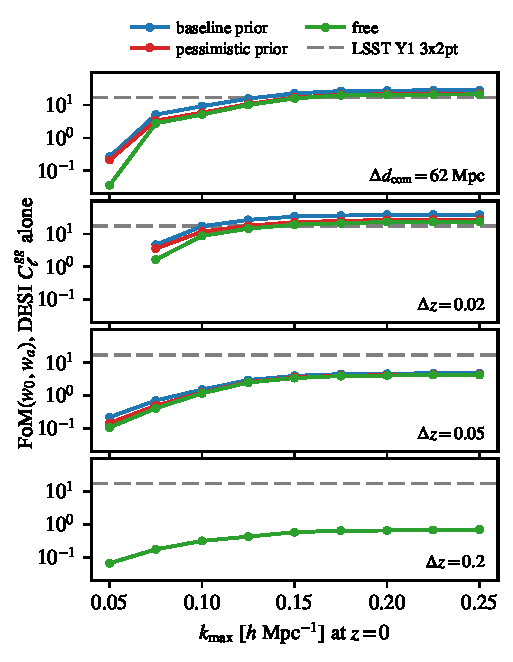
\includegraphics[width=3.5in]{plots/fom_kmax/fom_kmax.pdf}
  \caption{${\rm FoM}(w_0, w_a)$ of a linear-bias fit to the DESI
    $C_\ell^{gg}$ alone against the scale cut, one panel per layout,
    for the priors that pass the accuracy test.  Gray dashed line: the
    LSST Y1 3x2pt FoM.  On $\Delta z = 0.02$ the cut at $0.05$ keeps
    no band; on $\Delta z = 0.2$ the three priors coincide.
    \kmaxclause}
  \label{fig:fomkmax}
\end{figure}

\clearpage

\appendix

\section{Method}
\label{app:method}

\subsection{The truths}
\label{sec:truths}

Each truth is a full model A data vector at the project's fiducial
cosmology, with the linear biases at their fiducial values
$b_{1,i} = B_g/D(\bar{z}_i)$.  The calibrated truth uses the Lazeyras
et al.\ separate-universe fit \cite{Lazeyras2016},
$b_2(b_1) = 0.412 - 2.143\,b_1 + 0.929\,b_1^2 + 0.008\,b_1^3$, and
the co-evolution value $b_{s^2} = -\tfrac{4}{7}(b_1 - 1)$ of a
population formed with local bias and moved by gravity
\cite{Saito2014}.  The brackets $b_2 \pm 1$ set every group's offset
$\Delta_{2,g} = b_2 - b_2(b_1)$ to $\pm 1$.  The brackets
$\alpha_0 = \pm 12.5\,h^{-2}\,{\rm Mpc}^2$ put that counterterm in
every group: $\alpha_0 k^2 = 0.5$ at $k = 0.2\hMpc$, a $50\%$
correction there \cite{Maus2024}.  CosmoLike's counterterm slot is
$2\,b_1 b_K\,k^2 P_{\rm mm}$, with $b_K$ its per-bin derivative-bias
coefficient, so $\alpha_0 = 2\,b_1 b_K\,(c/H_0)^2$.

The vectors use the accuracy settings of the cached linear
derivatives and the exact white-noise split of CosmoLike's low-rank
engine.  That engine factorizes $P_{gg} - P_\infty$, where $P_\infty$
is the negative white-noise constant that the subtracted loop terms
tend to at high $k$; $P_\infty$ reaches $C_\ell$ through Limber, which
is exact for a constant (\texttt{notes/higher\_order\_bias}, subsection
``The white-noise limit of the renormalized loops'').

\subsection{The fit: linear response under each prior}
\label{sec:response}

Let $m$ be the expected data vector, $\Cov$ its covariance on the
kept entries (its inverse rescaled from $14{,}000$ to $12{,}300$
square degrees), and $\mathsf{D} = \partial m/\partial p$ the
derivatives of the linear-bias model with respect to the fitted
parameters $p$: the seven cosmological parameters ($10^9 A_s$, $n_s$,
$H_0$, $\Omega_b$, $\Omega_m$, $w_0$, $w_a$, flat priors), the bias
parameters of the prior, and the per-group velocity dispersions with
their Gaussian priors.  The fit's Fisher matrix is
$F = \mathsf{D}\T \Cov^{-1} \mathsf{D} + F_{\rm priors}$, where
$F_{\rm priors}$ holds the velocity-dispersion priors and, for the
baseline and pessimistic priors, the projected precision of the bias
prior (the correlated-prior note, sections ``The projected precision
for two bins'' and ``The memory model'').

If the data are the truth $m_{\rm truth}$ while the model at the
fiducial predicts $m_{\rm lin}$, then to first order the best fit
moves by
\begin{equation}
  \delta p \;=\; F^{-1}\,\mathsf{D}\T\, \Cov^{-1}
  \bigl(m_{\rm truth} - m_{\rm lin}\bigr) .
  \label{eq:response}
\end{equation}
At the old best fit the gradient of the log posterior becomes
$\mathsf{D}\T \Cov^{-1}(m_{\rm truth} - m_{\rm lin})$ instead of zero,
and $F$, the curvature, converts that gradient into a parameter
displacement.  The growth-tied prior uses the cached growth-tied
derivatives, one bias column per group; the other priors use the
per-bin derivatives, one column per bin.  Both come from the linear
notebook, \texttt{EXAMPLE\_EVALUATE\_FISHER.ipynb}.

\subsection{The scores and the threshold}
\label{sec:scores}

With $\delta w$ the $(w_0, w_a)$ entries of $\delta p$ and $\Cov_w$
the $(w_0, w_a)$ block of $F^{-1}$, the $(w_0, w_a)$ shift is
\begin{equation}
  \Delta_w \;=\; \sqrt{\delta w\T\, \Cov_w^{-1}\, \delta w} ,
  \label{eq:shiftw}
\end{equation}
the displacement of the dark-energy ellipse in units of its own size.
For one parameter $p$ the shift is $\Delta_p = |\delta p|/\sigma_p$,
with $\sigma_p = \sqrt{(F^{-1})_{pp}}$.  A shift of $\sigma/3$ added
in quadrature to a $1\sigma$ error gives $\sqrt{1 + 1/9} = 1.05$:
below the threshold the total error grows by at most about $5\%$.

\subsection{Cuts without data and the safe $\kmax$}
\label{sec:cut}

At each $\kmax$ the inverse covariance is rebuilt on the kept entries.
The shipped mask's cap, $0.1185\,{\rm Mpc}^{-1}$, is about
$0.176\hMpc$ at the fiducial $h = 0.6732$; at the largest cuts it,
not Eq.~\eqref{eq:uvfraction}, sets more and more of the kept bands,
and the curves of Figures~\ref{fig:fobkmax} and~\ref{fig:fomkmax}
flatten.

At small $\kmax$ some bins lose every band, and their bias columns
hold only finite-difference noise.  A parameter whose information
(data and prior) at a cut is below $10^{-10}$ of its information on
the full shipped mask therefore leaves the fit at that cut.  A cut
that leaves no data for the cosmological parameters gives no fit, as
on $\Delta z = 0.02$ at $\kmax = 0.05\hMpc$.  The safe $\kmax$ of
Table~\ref{tab:safe} is the largest scanned cut at which every score
of every truth considered is below $1/3$, at that cut and at every
smaller cut with a fit; a cut without a fit is skipped.

\section{Numerical checks}
\label{app:checks}

\begin{itemize}
  \item \textbf{One fiducial vector.}  The linear vector computed with
    the truths equals the cached reference of the linear notebook
    exactly on $\Delta d_{\rm com} = 62$~Mpc, $\Delta z = 0.02$ and
    $0.05$.  On $\Delta z = 0.2$ the largest relative difference,
    $4.5\times10^{-3}$, sits at a cross spectrum with nearly zero band
    powers; the median is $2\times10^{-5}$, and
    $\Delta\chi^2 = 2\times10^{-5}$ on the shipped mask.
  \item \textbf{Size of the one-loop sector.}  The one-loop part of
    the calibrated truth is a median $1.9\%$, $1.6\%$, $2.3\%$ and
    $1.9\%$ of the linear band powers on $\Delta d_{\rm com} = 62$~Mpc,
    $\Delta z = 0.02$, $0.05$ and $0.2$.
  \item \textbf{The truths of the accuracy test.}  The drifts and the
    $2000$ random truths are drawn with the linear notebook's seed and
    in its order: they are the truths the correlated-prior note fits
    under model A.  When the fit's prior equals the truth's scatter,
    the scatter and noise terms of $\langle\chi^2_w\rangle$ must sum
    to exactly $2$; they do to $1.6\times10^{-10}$.  The $(w_0, w_a)$
    value of $\chidof$ is then within $0.03$ of $1$, the remainder
    being the drift.
  \item \textbf{The white-noise constant.}  The exact projection of
    the one-loop white-noise constant leaves linear-bias vectors
    bitwise unchanged (\texttt{notes/higher\_order\_bias}).
\end{itemize}

\section{Limitations}
\label{app:limits}

\begin{itemize}
  \item \textbf{Linear response.}  The shifts are the first-order
    response of Eq.~\eqref{eq:response}, not a nonlinear refit.  Most
    verdicts rest on shifts well below the threshold or several times
    above it; a refit could move the cases near it, on
    $\Delta z = 0.05$ and $0.2$ at $0.05$ and growth-tied on
    $\Delta z = 0.2$ at $0.075$ ($0.40\sigma$).
  \item \textbf{Theory truths, not mocks.}  The truths are model A at
    and around its calibrations; a sample whose higher-order biases
    sit outside the brackets is not covered.
  \item \textbf{No stochastic term.}  The truths carry no non-Poisson
    shot noise and set $b_3 = 0$.  The effect of a constant noise
    power, which projects to an $\ell$-independent $C_\ell$, is not
    measured.
  \item \textbf{Real-space loops.}  The truths add only the real-space
    one-loop terms of model A; the redshift-space one-loop terms of
    model B are absent from truth and fit alike.
  \item \textbf{Negative power in one bracket.}  For BGS-like $b_1$
    the $\alpha_0 = -12.5\,h^{-2}\,{\rm Mpc}^2$ truth makes $P_{gg}$
    negative above $k \approx 0.37\hMpc$, where the low-rank
    non-Limber correction floors it; this is immaterial at
    $\kmax \le 0.075\hMpc$.
\end{itemize}

\section{Open issues}
\label{app:open}

\begin{itemize}
  \item \textbf{The covariance carries linear bias only.}  Its signal
    is the linear-bias $C_\ell^{gg}$ with $b_i = B_g/D(\bar{z}_i)$;
    the one-loop terms of model A are left out.  They are a median
    $1.6$--$2.3\%$ of the band powers (Appendix~\ref{app:checks});
    their effect on the errors is not measured here.
  \item \textbf{The cut was built on the linear model.}
    Eq.~\eqref{eq:uvfraction} is evaluated on linear-bias band powers.
    The counterterm, with its $k^2$ weight, draws more of its signal
    from beyond the cut: on $\Delta z = 0.05$ at $0.075\hMpc$ the
    ultraviolet fraction of the $\alpha_0$ template is a median
    $0.076$ on the kept bands, above $\alpha$, while for the full
    model A vector it is a median $0.017$ and at most $0.052$ (the
    correlated-prior note, subsection ``Open: the counterterm's share
    beyond the cut'').
\end{itemize}

\begin{thebibliography}{99}

\bibitem{Saraivanov2026}
E. Saraivanov, H. Rubira, V. Miranda and T. Eifler,
``Towards the Two-Loop EFTofLSS in Galaxy Lensing Surveys'',
2026, arXiv:2603.13031.

\bibitem{DeRoseChen2025}
J. DeRose and S. Chen,
``The Lensing Counter Narrative: An Effective Description of
Small-Scale Clustering in Weak Lensing Power Spectra'',
2025, arXiv:2510.18981.

\bibitem{Lazeyras2016}
T. Lazeyras, C. Wagner, T. Baldauf and F. Schmidt,
``Precision measurement of the local bias of dark matter halos'',
2016, arXiv:1511.01096.

\bibitem{Saito2014}
S. Saito, T. Baldauf, Z. Vlah, U. Seljak, T. Okumura and P. McDonald,
``Understanding higher-order nonlocal halo bias at large scales by
combining the power spectrum with the bispectrum'',
2014, arXiv:1405.1447.

\bibitem{DESI2024V}
DESI Collaboration,
``DESI 2024 V: Full-shape galaxy clustering from galaxies and
quasars'',
2024, arXiv:2411.12021.

\bibitem{Maus2024}
M. Maus, S. Chen, M. White et al.,
``An analysis of parameter compression and full-modeling techniques
with Velocileptors for DESI 2024 and beyond'',
2024, arXiv:2404.07312.

\end{thebibliography}

\end{document}
